\section{Evaluation}
\label{sec:eval}


\subsection{Evaluation Data Sets}
\label{sec:eval:data}


We prepare two data sets by extracting Quack test records from Censored 
Plant~\cite{sundara_raman_censored_2020}. One data set is for training and
evaluating the latent feature learning model while the other for training and
evaluating censorship detection.  For convenience, we refer to the
former data set as Data Set FL while the later Data Set CD. 

It is important to note that Censored Planet organizes their data based on
tests it runs. Specifically, each test is defined by its test request sent
from a vantage point, and this test is to run multiple times, which results in
multiple responses for the same test request message. On Censored Planet, a
record consists of the metadata about the test request message and the
multiple response messages. We flatten each Censored Planet test record by
iteratively pairing the top level request metadata with each response message
to create a record, essentially a record akin to a single request-response pair. 
This is to
match the intended use of the system, i.e., for each request sent, we want to
determine whether the request is censored based on the response received. In
the remainder of this article, a test record is like a request-response pair as described,
rather than a test record on Censored Planet.


Data Set FL
consists of \FLnrecords response records of the tests that Censored Plant ran
while Data Set CD consists of \CDnrecords vectors created as described in Section \ref{sec:design:vector} paired with metadata. The metadata consists of the domain or string under test, the IP address and country of the vantage point, timestamp for the test, and a flag value for censored, uncensored or undetermined. 


Censored Planet matches each test response with a censorship fingerprint
written in regular expression~\cite{sarah_laplante_blockpage_2021} and assigns
a label to each test record. The label can be either ``censored'', ``uncensored'',
or ``undetermined''. It is worth noting that the latent feature representation
learning model in Section~\ref{sec:design:fl} is an unsupervised learning
model, as such, the label is irrelevant and unused. However, the censorship
classification model in Sections~\ref{sec:design:cd}
and~\ref{sec:design:alternate} are supervised models and the labels are
necessary for training and also serve as the ``ground truth'' for evaluation.

Table~\ref{tab:data} summarizes useful statistics for the two data sets. 
\begin{table}[!htbp]
	\centering
	\caption{Evaluation Data Sets}
	\label{tab:data}

	\begin{tabular}{p{0.67\columnwidth} r}
		\toprule
		\multicolumn{2}{c}{Data Set FL (for Feature Learning)} \\
		\midrule
		\# of Training Records & \FLntrain \\
		\# of Validation Records & \FLnvalid \\
		Total  & \FLnrecords \\
		\midrule
		\multicolumn{2}{c}{Data Set CD (for Censorship Detection)} \\
		\midrule
		\# of Censored Records & \CDncensored \\
		\# of Uncensored Records & \CDnuncensored \\
		\# of Undetermined Records & \CDnunknown \\
		Total & \CDnrecords \\
		\bottomrule
	\end{tabular}
\end{table}

\subsection{Baseline Model}
\label{sec:eval:dense}
We treat the alternative model in Section~\ref{sec:design:alternate} as 
a baseline mode, and discuss its evaluation first here. 
We expand the vector in each record in Data Set CD to an vector of length $224
\times 224$ by padding each end
of the byte sequence with zeros if necessary, export the vector to bytes
and treat each vector as a gray-scale image. 
The training and evaluating settings are similar to those for the 
CD Classifier discussed in Section~\ref{sec:eval:cd:train} later.  
These include the hold-out evaluation setting, i.e., we randomly partition
the data set into three partitions, \CDtrainratio of the data for training,
\CDvalidratio for validation, and \CDtestratio for testing. In addition, we use a learning
rate scheduler that varies the learning rate between $1 \times 10^{-6}$ and $1
\times 10^{-7}$. The scheduler is  a cosine annealing 
strategy~\cite{loshchilov10sgdr} with period of
10 epochs. We monitor the training processing using the validation loss and
accuracy as shown in
Figure \ref{fig:dn_val_loss} and Figure \ref{fig:dn_val_acc}. The trained
network resulted in a loss of 0.048 on the test data with an accuracy of 0.986
where the accuracy is defined $(TP + TN)/(P + N)$.

\begin{figure}[!htbp]
	\centering
	\begin{subfigure}[b]{0.8\columnwidth}
		\centering
		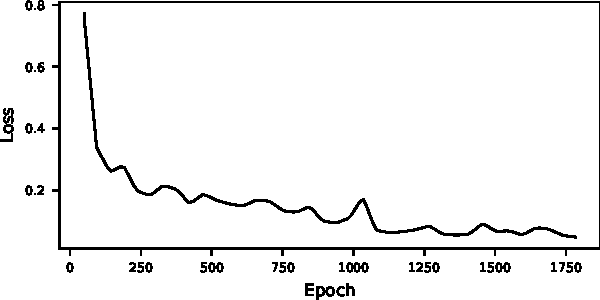
\includegraphics[width=\textwidth]{figures/densenet_validation_loss.pdf}
		\caption{Validation Loss}
		\label{fig:dn_val_loss}
	\end{subfigure}
	\hfill
	\begin{subfigure}[b]{0.8\columnwidth}
		\centering
		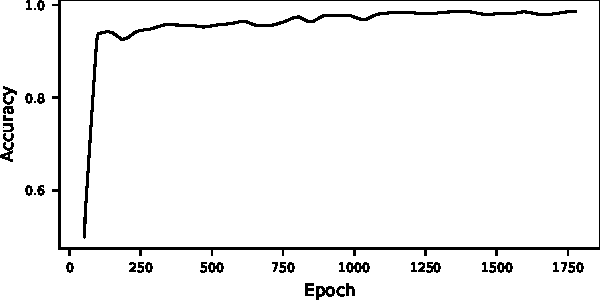
\includegraphics[width=\textwidth]{figures/densenet_validation_accuracy.pdf}
		\caption{Validation Accuracy}
		\label{fig:dn_val_acc}
	\end{subfigure}
	\caption{Validation loss and accuracy over training epochs}
	\label{fig:dn:train}
\end{figure}

\subsection{Feature Representation Learning}
The Censor2Seq model described in Section~\ref{sec:design:fl} is to learn
latent feature representation.  Table~\ref{tab:fl:params} summarizes the
hyperparameters of the Censor2Seq model used in this evaluation.  


To evaluate the latent feature representation learning model, we use Data Set
FL that is divided into a training and a validation data set (Table~\ref{tab:data}).  
Following the procedure in Section~\ref{sec:design:vector}, we convert
each test record in the data set to a sequence of numerical values
represented as a numerical vector. This process is described in Section~\ref{sec:design:vector}
in which we detail how the largest token value in our vectors is 7,069. This value is used to define
the embedding range.
% The size of each numerical vector is \FLseqlen.

For embedding size, we experiment with a
number of values with a consideration on memory requirement, processing time,
and convergence, find that the acceptable values range from \FLembsizemin
to \FLembsizemax, and settle at size \FLembsize.

\begin{table}[h]
	\centering
  \caption{Hyperparameters of Censor2Seq Model}
  \label{tab:fl:params}
	\begin{tabular}{p{0.67\columnwidth} r}
    \toprule
		Hyperparameter & Value \\
		\midrule
		size of input sequence size & \FLseqlen \\
    embedding dimension & \FLembsize \\
		\midrule
    encoder hidden layer size & \FLenchidden \\
    encoder output layer size & \FLencoutput \\
		\midrule
    decoder input layer size & \FLdecinput \\
    decoder hidden layer size & \FLdechidden \\
		\midrule
		decoder output sequence size & \FLdecoutput \\
    \bottomrule
  \end{tabular}
\end{table}



As shown in Table~\ref{tab:data}, we partition the data set into two subsets,
one for training and the other for validation. To reduce the demand of
computational resources, such as, memory and CPU time, we adopt a statistical
gradient descent (SGD) mini-batch training approach where we randomly sample
\FLsamplingratio of training data, i.e., sample from \FLntrain records 
at each training
epoch and set batch size as \FLbatchsize. Following the best practice, we
select a simple learning rate scheduler that uses 
a cosine annealing strategy~\cite{loshchilov10sgdr}
that decays learning rate smoothly from \FLlrbegin to \FLlrend with period of
10 epochs.  


We monitor the training process by checking on the entropy loss function value
computed on the validation subset following each epoch. Following the selected
early exit strategy, we stop the training process when the validation entry
loss function value twice dipped below \FLlossthreshold of the initial entropy
loss. The validation loss function value over training epochs is in
Figure~\ref{fig:ae_val_loss}.

\begin{figure}[!htbp]
    \centering
    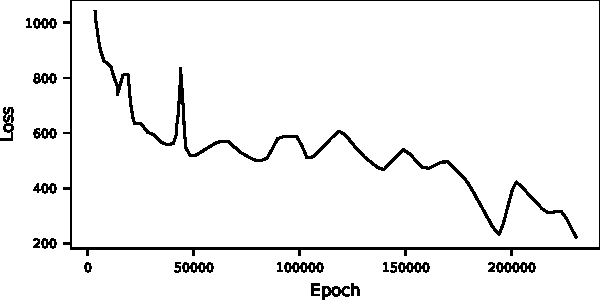
\includegraphics[width=0.8\columnwidth]{figures/autoencoder_val_loss.pdf}
    \caption{Validation loss of the Censor2Seq model.}
    \label{fig:ae_val_loss}
\end{figure}


The effectiveness of the Censor2Seq model is ultimately  reflected by the quality of
the lightweight numerical embeddings it produces.  In the Section~\ref{sec:eval:cd}, we evaluate how
effective the embeddings are to detect censorship events. 

\subsection{Censorship Detection}
\label{sec:eval:cd}

Section~\ref{sec:design:cd} describes the classifier for censorship detection.
It is a fully connected dense neural network. Table~\ref{tab:cd:params} is
the hyperparameters of the neural network. 
This neural network is a supervised classification model that requires
training.


\begin{table}[h]
	\centering
  \caption{Hyperparameter of Censorship Detection Neural Network}
  \label{tab:cd:params}
  \begin{tabular}{p{0.67\columnwidth} r}
    \toprule
    Parameter & \\
    \midrule
    input size & \CDinputsize \\ 
    first layer size & \CDfirstsize \\
    second layer size & \CDsecondsize \\
		output layer size & \CDoutputsize\\
    % \midrule
    % trainable parameters &  $2 \times 10^{6}$ \\
    \bottomrule
  \end{tabular}
\end{table}


\subsubsection{Training}
\label{sec:eval:cd:train}

We use Data Set CD to train the CD classifier. For each test record in Data Set
CD, we process it using the trained Censor2Seq model. As a result, we obtain an
embedding vector for each test record in Data Set CD. We adopt a
hold-out evaluation strategy where we randomly partition the data set
into three partitions, \CDtrainratio of the data for training, \CDvalidratio
for validation, and \CDtestratio for testing. 

As shown in Table~\ref{tab:data}, the censorship data here is unbalanced with
regard to its label where there are 3 times as many responses identified as
uncensored as those censored.  We applied an approach of under-sampling the
majority class to balance the training dataset whenever labeled data are
needed, i.e., during the training we randomly under-sample the training data
from the uncensored records, the majority class to match the censored records,
the minority class.


\begin{figure}[!htbp]
  \centering
	\begin{subfigure}[b]{0.8\columnwidth}
		\centering
		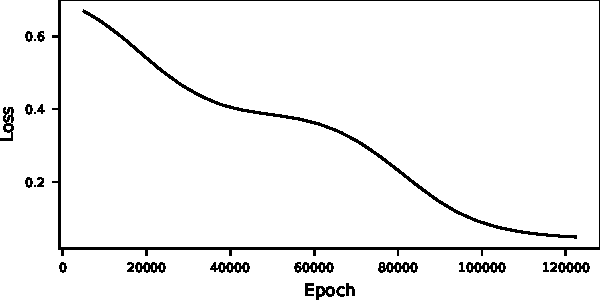
\includegraphics[width=\textwidth]{figures/le_val_loss.pdf}
		\caption{Validation Loss}
    \label{fig:le_val_loss}
	\end{subfigure}
	\hfill
	\begin{subfigure}[b]{0.8\columnwidth}
		\centering
		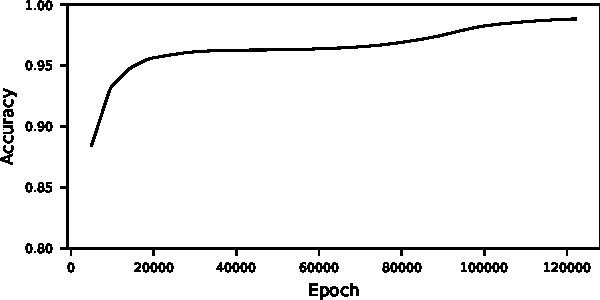
\includegraphics[width=\textwidth]{figures/le_val_acc.pdf}
		\caption{Validation Accuracy}
    \label{fig:le_val_acc}
	\end{subfigure}
	\caption{Validation loss and accuracy of the CD classifier over training epoch}
	\label{fig:cd:train}
\end{figure}

The learning rate scheduler uses a cosine annealing
strategy~\cite{loshchilov10sgdr} with the period of 10 epochs and varies the
learning rate between $1 \times 10^{-6}$ and $1 \times 10^{-7}$.  To prevent
overfitting, we check the entropy loss value computed on the validation data
after each training epoch and stop training when the validation loss ceases to
reduce. We aid this by using an early stopping strategy to eliminate
unnecessary excessive training time.  Figures \ref{fig:le_val_loss} and
\ref{fig:le_val_acc} illustrate the validation loss and the classification
accuracy over training epochs.  


\subsubsection{Testing}
Finally, to evaluate the effectiveness of the classifier, a surrogate to the
effectiveness of the embeddings produced by the trained Censor2Seq model, we
classify the test data set with the trained classifier. The classifier results
in a loss of $0.047$ and an accuracy of $0.988$ where the accuracy is
defined $(TP + TN)/(P + N)$. 


\begin{table}[!htbp]
	\centering
	\caption{Comparison of Classification Accuracy of E2ECD and DenseNetCD}
	\label{tab:eval:compare}
	\begin{tabular}{p{0.3\columnwidth} r r}
		\toprule
		Model & Loss & Accuracy \\
		\midrule
		E2ECD& 0.047 & 0.988 \\
		DenseNetCD & 0.048 & 0.986 \\
		\bottomrule
	\end{tabular}
\end{table}

Table~\ref{tab:eval:compare} summarizes and compares the evaluation results of
this model and the baseline model. The classification performance of the two
models are close if not considered identical. However, the E2ECD
model has a clear advantage when it comes to classifying
undetermined test records as discussed in Section~\ref{sec:eval:undermine}.

\subsection{Censorship Detection on Undetermined Records}\label{sec:results}
\label{sec:eval:undermine}

Data Set CD contains a \CDnunknown test records labeled as undermined as discussed
in Section~\ref{sec:eval:data}. 
%The undetermined data was not used in the training of the Censor2Seq model.
We are interested to know whether there are censorship
events in this set of undetermined test records. For this, we classify the
records using both the trained CD Classifier and
DenseNetCD models. There is a striking difference between the results
of the models as shown in Table~\ref{tab:eval:undetermine}. To interpret the 
result, it is necessary to understand the measurement tests performed by 
Centered Planet. 

\paragraph{Background} The data records in Data Set CD are from Quack 
tests~\cite{vandersloot2018quack}. Two major phases of a Quack test are 
``Retry'' and ``Control''. In the ``Retry'' phase, the platform has
an Echo request with a potentially offending payload repeatedly sent by 
a vantage point, e.g., sent 5 times with a delay in between. When all 
requests result in a failure, the platform carries out the Control phase
where the platform has an Echo request with an innocuous payload sent by
the vantage point. Only when this Echo request fails, the test declares
that there might be a network reachability problem due to network 
interference. 

Quack is effectively detecting the network reachability resulted from network
interference~\cite{vandersloot2018quack}. However, not all of the network 
interference detected by Quack is censorship, The exceptions include server-side
blocking errors (e.g., HTTP Status Code 403), page-not-found errors (e.g., HTTP
Status Code 404), and DDOS checks on some domains~\cite{raman_measuring_2020}, In 
addition, a recent investigation also indicates that some Censored Planet test 
requests were not sent successfully, which could also lead to unexpected responses~\cite{niaki2020iclab}.


\begin{table}[!htbp]
	\centering
	\caption{Comparison of Classification Results on Undetermined Tests}
	\label{tab:eval:undetermine}
	\begin{tabular}{p{0.3\columnwidth} r r}
		\toprule
		Model & Probable Censorship & Probable\% \\
		\midrule
		E2ECD & 557,492 & 66.14\%\\
		DenseNetCD & 183 & 0.02\%\\
		\bottomrule
	\end{tabular}
\end{table}

\paragraph{Analysis of the Results}
Which model is more accurate? Our answer is not definite; however, it is more
likely that the CD Classifier produces more meaningful results, in particular, 
when considering the design of Quack, we expect a significant proportion of 
the undetermined records should be the results of censorship. Aiming to confirm
this, we divided each of the results into
groups based on the patterns of the data records.  Table~\ref{tab:ae_results} 
summarizes the grouping of the
classification result of the E2ECD model while Table~\ref{tab:dn_results} that
of the DenseNetCD model.


The E2ECD model via the CD Classifier yields far more censorship detections. We
can confirm with a high confidence that some of these results are indeed 
probable censorship events. For instance, groups 1--3 and 5--7 in 
Table~\ref{tab:ae_results} are the block pages of Internet filters (or Firewalls), 
such as, Bitdefender, Cisco Meraki, and Seqrite Endpoint Security, and 
in total, the 1,184 responses that are likely actual
censorship block pages by examining the patterns of the these block
pages. Similarly,  the 122 responses in group 4 that are an \textit{HTTP Code 302} response
are also likely the result of censorship 

Most of the remaining records are likely the result of censorship.  
An investigation on the
Great Firewall of China indicates that both \textit{connection reset by peer}
and \textit{connection timed out} are among its observable
characteristics~\cite{shu_data_2014}.  As discussed in the above, 
the response to the request sent to
these vantage points have been verified with innocuous payloads, and therefore
it is very unlikely that the network has unexpectedly and repeatedly failed
during these specific queries.

Table~\ref{tab:dn_results} summarizes the grouping of the result of the
DenseNetCD model.  There are far fewer results shown and all of them are block
pages or \textit{HTTP Code 302}. Clearly the ability of the DenseNetCD model
to discover new censorship events is questionable. 

We hypothesize that the difference between the models lie at the distinction
of the designs of the two approaches. DenseNet is designed for per-pixel prediction models.
As indicated in a recent study~\cite{cheng2021per}, the state-of-the-art per-pixel 
classification model underperforms mask classification models in image semantic 
segmentation tasks where the
mask classification models disentangle the image partitioning and classification
aspects of image segmentation. There is a parallel when it comes to the two censorship
detection models we proposed. The E2ECD model separates the censorship detection
into two tasks, feature representation learning and censorship detection while the DenseNetCD 
model bundles the two together. Additionally, the encoding method used by Censorship2Seq is also designed
to encode the relationships between the individual tokens while an image classifier is intended
to be aware of clusters of pixels, it is less aware of connections between distant pixels. Due to the design of the feature 
representation learning model and the disentanglement of the two tasks, E2ECD fares better
than DenseNetCD, as a result of more generalizable feature presentation learned by Censorship2Seq. It
is also highly likely that the DenseNetCD model learned highly idiosyncratic features specific to 
the training data, resulting in poor generalizability, and notably the
phenomenon of this nature has also been reported in studies using deep
learning models in other areas, such as, vulnerability prediction~\cite{chakraborty2021deep}. 

\begin{table*}
	\centering
  \caption{Censorship Candidates from E2DCD}
  \label{tab:ae_results}
	{\footnotesize
  \begin{tabular}{r p{0.25\textwidth} r p{0.55\textwidth}}
    \toprule
		No. & Type & Frequency & Locations\\
    \midrule
		1. & ATT block page & 3 & United States \\
		2. & Bitdefender Alert Page block page & 1,133 & India, United States \\
		3. & Extra Safe Internet block page & 4 & Netherlands \\
		4. & HTTP code 302 & 122 & Belarus, China, Kazakhstan, Pakistan, Russia \\
		5. & Meraki block page & 1 & Singapore \\
		6. & Seqrite Endpoint Security block page & 37 & India \\
		7. & Net Protector block page & 6 & India \\
		8. & `Connection: close` message returned without block page & 10 & China, U.S. Virgin Islands, United States \\
		9. & `connection reset by peer' error & 542,083 & Bangladesh, Brunei, Canada, China, Colombia, Egypt, Ethiopia, Germany, Hong Kong, India, Iran, Ivory Coast, Kenya, Libya, Mexico, Oman, Pakistan, Poland, Qatar, Russia, Saudi Arabia, Singapore, South Korea, Syria, Taiwan, Turkey, United Arab Emirates, United States, Uzbekistan, Vietnam \\
		10. & `no route to host' error & 296 & Argentina, Australia, Bangladesh, Belgium, Brazil, Colombia, Czechia, Germany, Greece, India, Indonesia, Italy, Japan, Libya, Malaysia, Mexico, Moldova, Nepal, Poland, South Korea, Spain, Switzerland, Taiwan, Thailand, United Kingdom, United States \\
		11. & `connection timed out' error & 2,885 & Angola, Argentina, Austria, Bangladesh, Brazil, Burundi, Canada, China, Colombia, Czechia, Germany, Greece, Guadeloupe, India, Iran, Italy, Japan, Mexico, Netherlands, Nigeria, Philippines, Russia, South Africa, South Korea, Spain, Sweden, Switzerland, Taiwan, Turkey, U.S. Virgin Islands, Ukraine, United Kingdom, United States \\
		12. & `I/O timeout' error & 6,983 & Algeria, Armenia, Bangladesh, Belarus, Belgium, Brazil, Burundi, Canada, China, Egypt, Germany, Guam, Hong Kong, India, Indonesia, Iran, Kazakhstan, Kenya, Madagascar, Malaysia, Mexico, Netherlands, Nigeria, Oman, Pakistan, Paraguay, Qatar, Romania, Russia, Saudi Arabia, South Korea, Taiwan, Tanzania, Thailand, Turkey, United Kingdom, United States, Uzbekistan, Vietnam, Zambia \\
		13. & `network is unreachable' error & 18  & Indonesia, Poland \\
		14. & `connection refused' error & 3,007 & Bangladesh, Brazil, Chile, China, Colombia, Czechia, Egypt, France, Germany, Greece, India, Italy, Ivory Coast, Japan, Kenya, Mexico, Nepal, Pakistan, Peru, Poland, Russia, Singapore, South Africa, South Korea, Spain, Sri Lanka, Sweden, Taiwan, Thailand, Ukraine, United States \\
		15. & `echo response does not match echo request' and no other data & 904 & Algeria, Armenia, Bangladesh, Belarus, Belgium, Brazil, Burundi, Canada, China, Egypt, Germany, Guam, Hong Kong, India, Indonesia, Iran, Kazakhstan, Kenya, Madagascar, Malaysia, Mexico, Netherlands, Nigeria, Oman, Pakistan, Paraguay, Qatar, Romania, Russia, Saudi Arabia, South Korea, Taiwan, Tanzania, Thailand, Turkey, United Kingdom, United States, Uzbekistan, Vietnam, Zambia \\
  \bottomrule
\end{tabular}
	}
\end{table*}

\begin{table*}
	\centering
  \caption{Censorship Candidates from DenseNetCD}
  \label{tab:dn_results}
	{\footnotesize
	\begin{tabular}{r p{0.25\textwidth} r p{0.55\textwidth}}
    \toprule
		No. & Type & Frequency & Locations\\
    \midrule
		1. & ATT block page & 3 & United States \\
		2. & Bitdefender Alert Page block page & 116 & India, United States \\
		3. & Extra Safe Internet block page & 1 & Netherlands \\
		4. & HTTP code 302 & 62 & China, Kazakhstan, Pakistan, Russia \\
		5. & Meraki block page & 1 & Singapore \\
  \bottomrule
\end{tabular}
		}
\end{table*}

